\section{Dataset Overview}

\begin{figure}
\centering
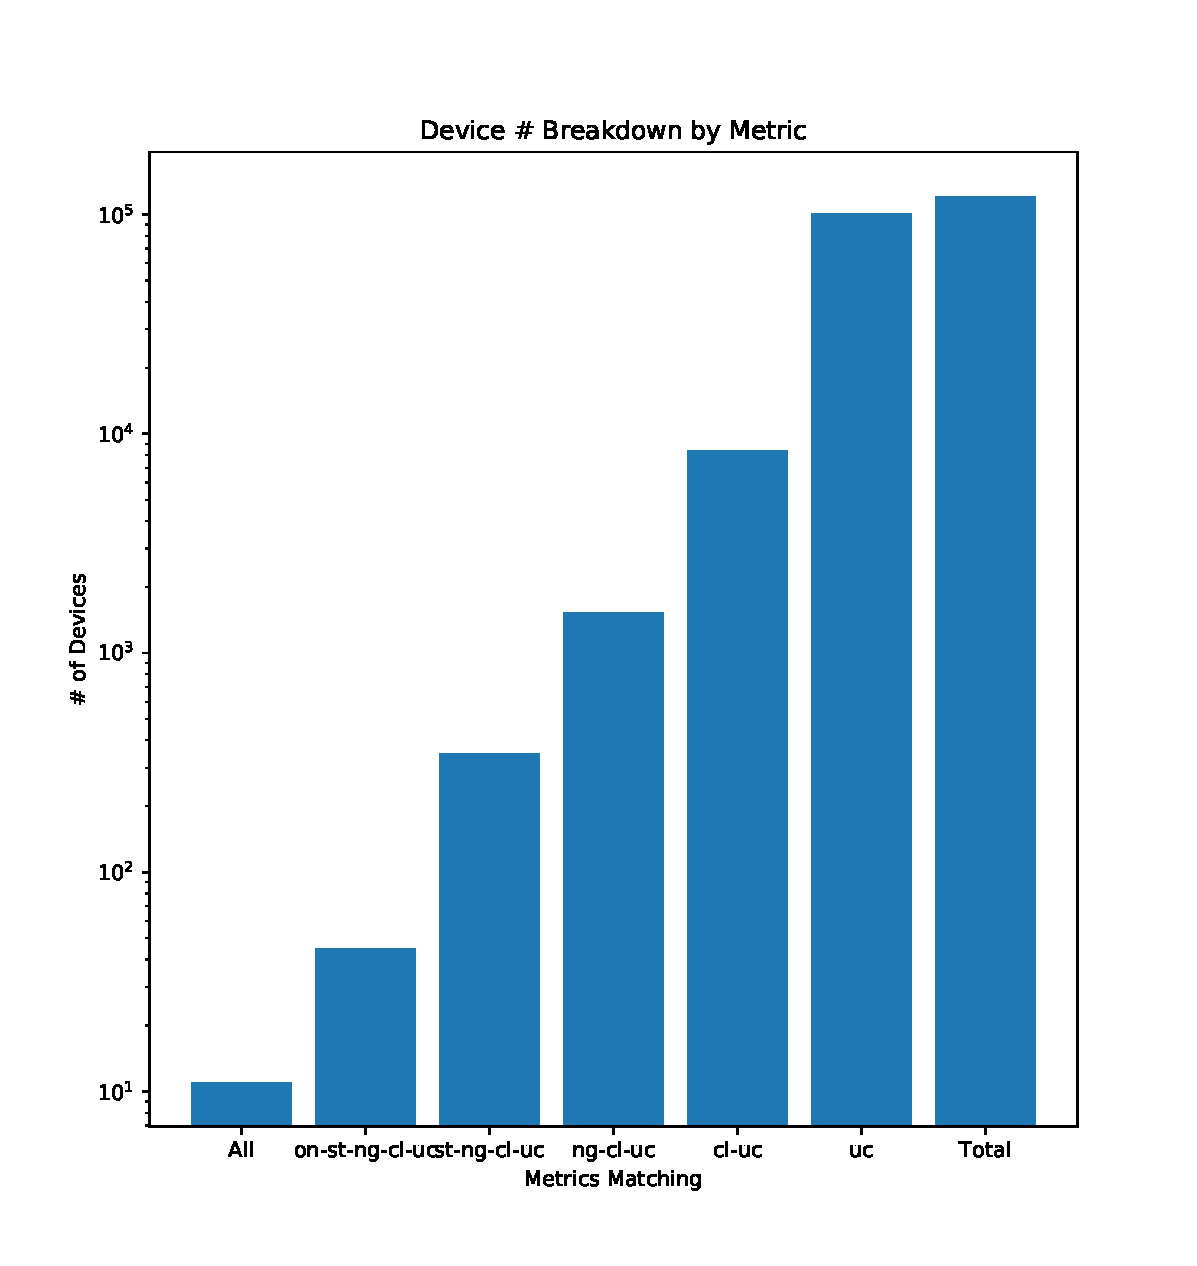
\includegraphics[width=\linewidth]{fig/dbstats}
\caption{
\label{fig:dbstats}
Bluetooth wardriving dataset overview \todo{Update with latest numbers}.
}
\end{figure}

We gathered inquiry responses from many gas stations in California, and created
simple filters for these fields to find devices that match the profile of one
of the wireless modules that can be used as a skimmer, and has been
seen before to be involved in skimmers (see our strategy for crowdsourced data
gathering for implant detection described in Section~\ref{sec:crowdsourcing}). 

Figure~\ref{fig:dbstats} shows an overview of the Bluetooth devices that we
observed.
%
\todo{Each field reduces the number of suspected implants by an order of
magnitude.}
%
This indicates that each field can be very useful in reducing the number of
potential implants. 
%
Figure~\ref{fig:dbstats} shows the results of this initial drive. Preliminary
Bluetooth scans around gas stations in California revealed 30,420 unique
Bluetooth MAC addresses, of which our preliminary Bluetooth-specific detection
techniques brought down to 70 likely targets, of which 4 were confirmed gas
station skimmers that were eventually recovered by the US Secret Service.

\section{Limitations}

\begin{enumerate}
\item  Unnamed Devices are a limitation
\item   We use the MAC address, other metrics in that case
\item   Method in field relies more on the hitlist
\item     Hitlist can be comprehensive
\item     Using data from police recovery, as well scraping of
    websites like alibaba, sparkfun, digifruit, ebay, ...
\item    	      Incremental; if a new device shows up and
	     we are notified, we can rerun metric analysis to
	     find the new hitlist devices
\item	      method is extendable
\item What about randomized MAC addreses / smarter skimmer
\item   Full randomization, the criminal must rely on the device name
  to recover the device, since the person that is extracting the
  data is not the same as the one that implanted. Crims generally
  use mules, according to law enforcement agencies.
\item   Now, there can be a limited randomization, in which you use
  a pool of MAC addresses
\item     This is more sophisticated, and damages our methodology, the
    mitigations for this are more complicated but come in one of
    two forms: either persistent monitoring devices at each gas station
    or an even larger crowd sourced approach, wherein you get enough coverage
    of each gas station to determine persistence
\item        This is more difficult to detect. You could flag based upon whether
       the MAC address device is abnormal compared to a baseline for other
       gas stations: if you see a thermostat, it is bad.
\item        But even apple uses 47 bits of randomization, trampling upon other
       manufacturers, so how do you tell this is not another consumer
       electronic, or that the criminal is not masquerading as a common
       bluetooth device, i.e. a Tile?
\item  So consider the case of a smart criminal (i.e. one of the authors of this
paper) designing a skimmer. They would randomize the fingerprint so that
it looks like one of 255 tiles.
\item    In a largescale crowdsourced approach, you might, in the best case,
   have someone come by and scan the gas station every 3 hours. Using our
   methodology, this would not flag odd name, bad MAC, seen twice ... 
\item    There is still a possibility! For each gas station, record the geoloc
   of each of the pumps. For each gas station, check the rssi of the devices
   scanned, and see get a high confidence localization inside the pump. From
   multiple datapoints, you should be able to determine whether the bluetooth
   device is inside of a pump, and there are no bluetooth devices commonly found
   inside pumps.
\item    and you can't spoof RSSI. It is approximate, and depends on the phone/reciever
\item    Since each phone has a subjective perspective, to get the ground truth, you
   would localize to a centroid for each observer, and then combine these centroids
   to localize the skimmer.
\item    Thus, even if criminals were not dumb, we could find them.
\end{enumerate}

